\documentclass[final,pdftex]{../../template/epsilonj}\usepackage[]{graphicx}\usepackage[]{color}
%% maxwidth is the original width if it is less than linewidth
%% otherwise use linewidth (to make sure the graphics do not exceed the margin)
\makeatletter
\def\maxwidth{ %
  \ifdim\Gin@nat@width>\linewidth
    \linewidth
  \else
    \Gin@nat@width
  \fi
}
\makeatother

\definecolor{fgcolor}{rgb}{0.345, 0.345, 0.345}
\newcommand{\hlnum}[1]{\textcolor[rgb]{0.686,0.059,0.569}{#1}}%
\newcommand{\hlstr}[1]{\textcolor[rgb]{0.192,0.494,0.8}{#1}}%
\newcommand{\hlcom}[1]{\textcolor[rgb]{0.678,0.584,0.686}{\textit{#1}}}%
\newcommand{\hlopt}[1]{\textcolor[rgb]{0,0,0}{#1}}%
\newcommand{\hlstd}[1]{\textcolor[rgb]{0.345,0.345,0.345}{#1}}%
\newcommand{\hlkwa}[1]{\textcolor[rgb]{0.161,0.373,0.58}{\textbf{#1}}}%
\newcommand{\hlkwb}[1]{\textcolor[rgb]{0.69,0.353,0.396}{#1}}%
\newcommand{\hlkwc}[1]{\textcolor[rgb]{0.333,0.667,0.333}{#1}}%
\newcommand{\hlkwd}[1]{\textcolor[rgb]{0.737,0.353,0.396}{\textbf{#1}}}%

\usepackage{framed}
\makeatletter
\newenvironment{kframe}{%
 \def\at@end@of@kframe{}%
 \ifinner\ifhmode%
  \def\at@end@of@kframe{\end{minipage}}%
  \begin{minipage}{\columnwidth}%
 \fi\fi%
 \def\FrameCommand##1{\hskip\@totalleftmargin \hskip-\fboxsep
 \colorbox{shadecolor}{##1}\hskip-\fboxsep
     % There is no \\@totalrightmargin, so:
     \hskip-\linewidth \hskip-\@totalleftmargin \hskip\columnwidth}%
 \MakeFramed {\advance\hsize-\width
   \@totalleftmargin\z@ \linewidth\hsize
   \@setminipage}}%
 {\par\unskip\endMakeFramed%
 \at@end@of@kframe}
\makeatother

\definecolor{shadecolor}{rgb}{.97, .97, .97}
\definecolor{messagecolor}{rgb}{0, 0, 0}
\definecolor{warningcolor}{rgb}{1, 0, 1}
\definecolor{errorcolor}{rgb}{1, 0, 0}
\newenvironment{knitrout}{}{} % an empty environment to be redefined in TeX

\usepackage{alltt}

\RequirePackage{graphicx}
\usepackage{verbatim}
\RequirePackage[colorlinks,citecolor=blue,urlcolor=blue]{hyperref}

\addbibresource{../../template/epsilon.bib}
\IfFileExists{upquote.sty}{\usepackage{upquote}}{}
\begin{document}
	
	\begin{frontmatter}
		\title{Распознавание рукописных цифр}
		\runtitle{Распознавание рукописных цифр}
		
		\begin{aug}
			\author{\imya{Саша} \fam{Кузнецова}}%
			
			\runauthor{Саша~Кузнецова}
			
			\address{НИУ ВШЭ, Москва.}
		\end{aug}
		
		\begin{abstract}
		Задача распознавания рукописного текста "--- одна из классических задач машинного обучения, к~решению которой применялось такое количество алгоритмов, что она успешно может быть использована в~качестве учебной. 
		
		В~этой заметке мы будем учиться распознавать написанные от руки цифры.
		\end{abstract}
		
		\begin{keyword}
			\kwd{k ближайших соседей}
			\kwd{R}
			\kwd{машинное обучение}
			\kwd{распознавание образов}
		\end{keyword}
		
	\end{frontmatter}
	
		
Мы обратимся к~одному из наиболее известных хранилищ, в~котором собраны обработанные изображения цифр, разберём, как эти данные оттуда извлекать, а~затем применим к~ним алгоритм $k$ ближайших соседей, используя \proglang{R}.
	
	\section{База данных MNIST}
	
Источником данных нам послужит база «MNIST» (\cite{mnistdigits}), \url{http://yann.lecun.com/exdb/mnist/}, в~которой хранятся 70\,000 изображений цифр, написанных несколькими сотнями разных людей. 
Каждая картинка в~этой базе обработана так, чтобы поместиться в~квадратик размером $28\times28$ пикселей. 
Каждый пиксель представлен числом от~0 до~255, где 0~соответствует белому цвету, а~255 "--- чёрному. 

Все изображения поделены на две части: 60\,000 относятся к~учебной выборке, а~10\,000 "--- к~тестовой. 
По учебной выборке наш алгоритм будет настраивать свои параметры, а~по тестовой мы будем оценивать качество классификации.
Такое разбиение нужно для того, чтобы убедиться, что алгоритм не переобучился, то есть не настроен исключительно на учебные примеры и~способен правильно классифицировать новые для него изображения.

Каждое из изображений в~нашей задаче должно быть отнесено к~одному из десяти классов "--- это цифры от~0 до~9. 
Для элементов обучающей выборки известно, к~какому классу они принадлежат, поэтому настройка параметров классифицирующего алгоритма относится к~области \textit{обучения с~учителем}. 
Это значит, что процесс обучения использует известные ответы и~стремится за счёт выбора параметров сделать предсказания алгоритма максимально близкими к~правильным (кстати, таким образом мы обучали все наши алгоритмы в~курсе эконометрики).

Как говорится, «наивные студенты думали, что .csv"=файлы на деревьях, как булки, растут», но всё оказалось совсем не так. 
Для того чтобы прочитать IDX-файл, в~котором хранятся данные с~изображениями цифр в~базе «MNIST», мне потребовались Google и~кандидат физико"=математических наук. 
Проблема заключается в~том, что данные хранятся в~этой базе в~бинарном виде, и~их не открыть в~привычных нам приложениях.
Вот как это можно сделать в~\proglang{R}.

\par\medskip
(1) Скачав данные с~сайта, открываем файл с~учебной выборкой на чтение командой \code|file|:

\begin{knitrout}
\definecolor{shadecolor}{rgb}{0.969, 0.969, 0.969}\color{fgcolor}\begin{kframe}
\begin{alltt}
\hlstd{to.read} \hlkwb{<-} \hlkwd{file}\hlstd{(}\hlstr{"train-images-idx3-ubyte"}\hlstd{,} \hlstr{"rb"}\hlstd{)}
\end{alltt}
\end{kframe}
\end{knitrout}

\par\medskip (2) Данные устроены таким образом, что в~самом начале мы читаем заголовок из четырёх чисел. Эти первые четыре числа содержат информацию о~размерах выборки, упомянутых выше. Считываем их из полученного объекта \code|to.read| с~помощью функции для чтения бинарных данных \code|readBin|.

\begin{knitrout}
\definecolor{shadecolor}{rgb}{0.969, 0.969, 0.969}\color{fgcolor}\begin{kframe}
\begin{alltt}
\hlkwd{readBin}\hlstd{(to.read,} \hlkwd{integer}\hlstd{(),} \hlkwc{n} \hlstd{=} \hlnum{4}\hlstd{,} \hlkwc{endian}\hlstd{=}\hlstr{"big"}\hlstd{)}
\end{alltt}
\begin{verbatim}
## [1]  2051 60000    28    28
\end{verbatim}
\end{kframe}
\end{knitrout}

\par\medskip (3) Далее для каждой картинки следуют $28\times28$ байт, содержащие информацию о~цвете каждого пикселя (числа от~0 до 255) и~записанные из изображения построчно. 
Получаем большой массив \code|TRAIN| из 60\,000 таблиц размером $28\times28$: берём первые 28 чисел и~кладём их в~первый столбец первой таблицы, продолжаем, пока не дойдём до 28-го столбца, затем приступаем к~следующей таблице "--- и~так до конца. 

Нужно обратить внимание, что изначально данные были разложены в~строку, но мы только что разложили их по столбцам, для того чтобы позже было удобнее выводить рисунок.

\begin{knitrout}
\definecolor{shadecolor}{rgb}{0.969, 0.969, 0.969}\color{fgcolor}\begin{kframe}
\begin{alltt}
\hlstd{TRAIN} \hlkwb{<-} \hlkwd{array}\hlstd{(}\hlkwc{data} \hlstd{=} \hlnum{NA}\hlstd{,} \hlkwc{dim} \hlstd{=} \hlkwd{c}\hlstd{(}\hlnum{28}\hlstd{,}\hlnum{28}\hlstd{,}\hlnum{60000}\hlstd{))}

\hlkwa{for}\hlstd{(i} \hlkwa{in} \hlnum{1}\hlopt{:}\hlnum{60000}\hlstd{)}
  \hlstd{\{}
\hlstd{TRAIN[,,i]} \hlkwb{<-} \hlkwd{matrix}\hlstd{(}\hlkwd{readBin}\hlstd{(to.read,}\hlkwd{integer}\hlstd{(),} \hlkwc{size} \hlstd{=} \hlnum{1}\hlstd{,}
    \hlkwc{n} \hlstd{=} \hlnum{28}\hlopt{*}\hlnum{28}\hlstd{,} \hlkwc{signed} \hlstd{=} \hlnum{FALSE}\hlstd{,} \hlkwc{endian} \hlstd{=} \hlstr{"big"}\hlstd{),} \hlnum{28}\hlstd{,} \hlnum{28}\hlstd{);}
  \hlstd{\}}
\hlkwd{close}\hlstd{(to.read)}
\end{alltt}
\end{kframe}
\end{knitrout}

\par\medskip (4) Перед тем как начинать работать с~данными и~оценивать по ним какие-либо модели, обычно бывает полезно взглянуть на них и~построить описательные статистики. В~данном случае для этой цели может послужить сама картинка.

\begin{knitrout}
\definecolor{shadecolor}{rgb}{0.969, 0.969, 0.969}\color{fgcolor}\begin{kframe}
\begin{alltt}
\hlkwd{layout}\hlstd{(}\hlkwd{matrix}\hlstd{(}\hlkwd{c}\hlstd{(}\hlnum{1}\hlopt{:}\hlnum{36}\hlstd{),} \hlnum{6}\hlstd{,} \hlnum{6}\hlstd{,} \hlkwc{byrow} \hlstd{=} \hlnum{TRUE}\hlstd{),}
   \hlkwc{widths} \hlstd{=} \hlkwd{lcm}\hlstd{(}\hlkwd{rep}\hlstd{(}\hlnum{2.5}\hlstd{,}\hlnum{36}\hlstd{)),} \hlkwc{heights} \hlstd{=} \hlkwd{lcm}\hlstd{(}\hlkwd{rep}\hlstd{(}\hlnum{2.5}\hlstd{,}\hlnum{36}\hlstd{)))}
\hlkwd{par}\hlstd{(}\hlkwc{mar}\hlstd{=}\hlkwd{c}\hlstd{(}\hlnum{0}\hlstd{,}\hlnum{0}\hlstd{,}\hlnum{0}\hlstd{,}\hlnum{0}\hlstd{))}

\hlkwa{for}\hlstd{(i} \hlkwa{in} \hlnum{1}\hlopt{:}\hlnum{36}\hlstd{)}
  \hlstd{\{}
\hlkwd{image}\hlstd{(TRAIN[,}\hlnum{28}\hlopt{:}\hlnum{1}\hlstd{,i])}
  \hlstd{\}}
\end{alltt}
\end{kframe}
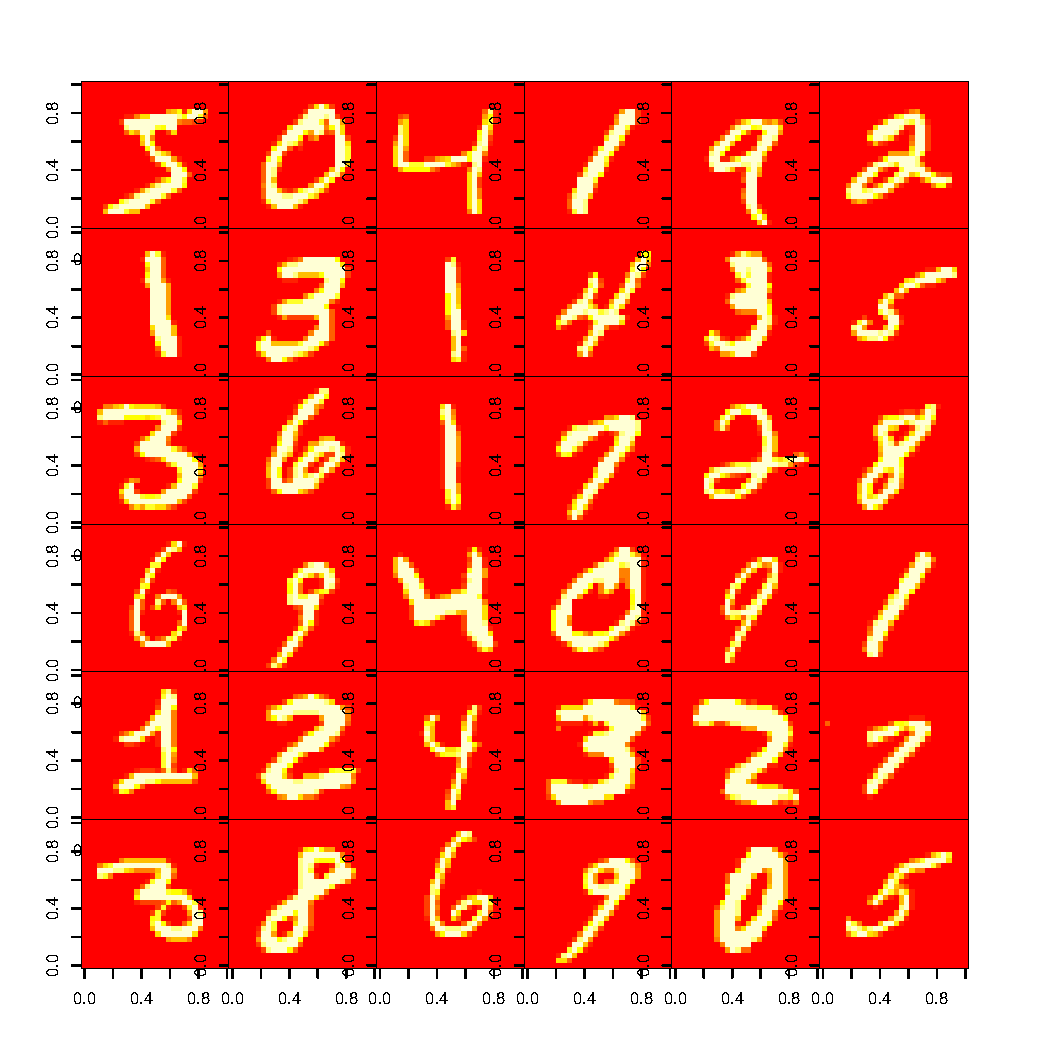
\includegraphics[width=\maxwidth]{figure/unnamed-chunk-4-1} 

\end{knitrout}

Нарисуем цифры по первым 36~таблицам из массива \code|TRAIN|. 
Нужно обратить внимание, что, нарисуй мы сейчас всё как есть, мы бы получили перевёрнутые цифры (это можно проверить), потому что функция \code|image| будет соотносить первый столбец с~нулевой ординатой на картинке, но мы помним, что первый столбец соответствовал верхней строке рисунка. 
Для того чтобы избежать этой проблемы, будем рисовать столбцы в~обратном порядке, от 28-го к~1-му: \code|TRAIN[,28:1,]|.

\par\medskip (5) Описанную выше процедуру повторяем, чтобы считать метки классов для учебной выборки. 
Заголовок в~данном случае состоит из двух чисел, а~данные должны восприниматься \proglang{R}'ом не как числа, а~как категории: этого можно добиться с~помощью команды \code|as.factor|.

\begin{knitrout}
\definecolor{shadecolor}{rgb}{0.969, 0.969, 0.969}\color{fgcolor}\begin{kframe}
\begin{alltt}
\hlstd{to.read} \hlkwb{<-} \hlkwd{file}\hlstd{(}\hlstr{"train-labels-idx1-ubyte"}\hlstd{,} \hlstr{"rb"}\hlstd{)}
\hlstd{header} \hlkwb{<-} \hlkwd{readBin}\hlstd{(to.read,} \hlkwd{integer}\hlstd{(),} \hlkwc{n}\hlstd{=}\hlnum{2}\hlstd{,} \hlkwc{endian}\hlstd{=}\hlstr{"big"}\hlstd{)}
\hlstd{Train_labels} \hlkwb{<-} \hlkwd{readBin}\hlstd{(to.read,} \hlkwd{integer}\hlstd{(),} \hlkwc{size} \hlstd{=} \hlnum{1}\hlstd{,}
            \hlkwc{n} \hlstd{=} \hlnum{60000}\hlstd{,} \hlkwc{signed} \hlstd{=} \hlnum{FALSE}\hlstd{,} \hlkwc{endian}\hlstd{=}\hlstr{"big"}\hlstd{)}
\hlstd{Train_labels} \hlkwb{<-} \hlkwd{as.factor}\hlstd{(Train_labels)}
\hlkwd{close}\hlstd{(to.read)}
\end{alltt}
\end{kframe}
\end{knitrout}

\par\medskip
Итак, на данном этапе мы являемся обладателями учебной выборки (но умеем читать и~многое другое) и~великолепной картинки, что означает, что пора бы с~ними что-нибудь да~сделать. 

\section{Алгоритм $k$ ближайших соседей}

Одним из простейших алгоритмов классификации является метод $k$ ближайших соседей (\ENGs{$k$ Nearest Neighbours}, kNN). 
Основной идеей данного алгоритма является то, что объект, как правило, находится в~окружении объектов своего же класса. 
Таким образом, чтобы классифицировать новый объект, мы должны посмотреть на $k$ ближайших к~нему объектов из учебной выборки и~отнести его к~тому классу, который среди них чаще встретился.

Первый вопрос, который перед нами встаёт, "--- это выбор функции расстояния между объектами выборки.
В~простом случае, когда объекты представлены в~виде числовых векторов, пользуются простой евклидовой метрикой, то есть $\rho(a, b) = \sqrt{\sum\limits_{k = 1}^m(a_k-b_k)^2}$.

Второй проблемой является выбор значения $k$: сколько объектов нам нужно посмотреть, чтобы наиболее точно классифицировать наш? 
Единого правила для того, чтобы выбрать $k$, не существует, однако нужно учитывать, что при слишком маленьких $k$ алгоритм будет неустойчивым, а~при слишком больших начнёт подстраиваться к~шуму и~терять обобщающую способность. 
Конкретное значение $k$ можно определить опытным путём: попробовать диапазон значений и~посмотреть, какое подходит лучше.

\subsection{Существующие реализации}

Для реализации алгоритма $k$ ближайших соседей в~\proglang{R} есть как минимум три пакета: \pkg{kknn}, \pkg{FNN} и~\pkg{RWeka}, причём в~двух последних есть ещё и~готовые базы данных.

Пакет \pkg{kknn} реализует алгоритм kNN с~весами, где голоса «соседей» не равнозначны, а~входят в~общую сумму с~определёнными весами. Мы его реализовывать не будем.

Воспользуемся функцией \code|install.packages(c("FNN", "RWeka"))|, чтобы загрузить пакеты.

\subsection{Пакет \pkg{FNN}}

Воспользуемся теперь пакетом \pkg{FNN} (\cite{RFNNpackage14}), предварительно проделав с~данными для тестовой выборки то же, что и~с~учебными, в~итоге получив два больших массива, \code|TRAIN| и~\code|TEST|, а~также два вектора ответов, \code|Trainlabels| и~\code|Testlabels|. 



Функция \code|knn| пакета \pkg{FNN} в~качестве аргументов принимает матрицы учебных и~тестовых данных, а~также вектор ответов для тренировочной выборки, а~на выходе отдаёт предсказанную классификацию для тестовой выборки. 
Эта функция сразу и~обучается, и~предсказывает "--- очень удобно.

Сейчас наши данные выглядят не так, как нужно этой функции, поэтому преобразуем их в~матрицу, содержащую значения цвета всех пикселей, размещённых в~одну строку для каждой картинки. 
Воспользуемся функцией \code|as.vector|, которая будет по очереди брать столбцы из матрицы и~выкладывать их в~одну строку. 
Кроме того, для примера мы будем использовать только первую тысячу наблюдений из учебной выборки и~пятьсот из тестовой. 
Если читатель желает получить более точный классификатор, то в~этом месте следует использовать все 60\,000 и~10\,000 соответственно.

\begin{knitrout}
\definecolor{shadecolor}{rgb}{0.969, 0.969, 0.969}\color{fgcolor}\begin{kframe}
\begin{alltt}
\hlstd{n} \hlkwb{<-} \hlnum{1000}
\hlstd{train} \hlkwb{=} \hlkwd{matrix}\hlstd{(}\hlkwc{data} \hlstd{=} \hlnum{NA}\hlstd{,} \hlkwc{nrow} \hlstd{= n,} \hlkwc{ncol} \hlstd{=} \hlnum{28}\hlopt{*}\hlnum{28} \hlstd{)}

\hlkwa{for} \hlstd{(i} \hlkwa{in} \hlnum{1}\hlopt{:}\hlstd{n)}
  \hlstd{\{}
\hlstd{train[i,]} \hlkwb{<-} \hlkwd{as.vector}\hlstd{(TRAIN[,,i])}
  \hlstd{\}}
\hlstd{train_labels} \hlkwb{<-} \hlstd{Train_labels[}\hlnum{1}\hlopt{:}\hlstd{n]}
\end{alltt}
\end{kframe}
\end{knitrout}



Теперь воспользуемся функцией \code|knn|, чтобы классифицировать объекты тестовой выборки, и запишем результаты в~вектор \code|results|. Возьмём, например, $k=10$. 
Преимуществом функции является высокая скорость подсчёта предсказаний.

\begin{knitrout}
\definecolor{shadecolor}{rgb}{0.969, 0.969, 0.969}\color{fgcolor}\begin{kframe}
\begin{alltt}
\hlkwd{library}\hlstd{(FNN)}
\hlstd{results} \hlkwb{<-} \hlstd{(}\hlnum{0}\hlopt{:}\hlnum{9}\hlstd{)[}\hlkwd{knn}\hlstd{(train, test, train_labels,} \hlkwc{k} \hlstd{=} \hlnum{10}\hlstd{,}
                     \hlkwc{algorithm} \hlstd{=} \hlstr{"cover_tree"}\hlstd{)]}
\end{alltt}
\end{kframe}
\end{knitrout}

Посмотрим на долю ошибок, которые мы допустили при классификации. 
Она достаточно высока, но это можно объяснить тем, что мы использовали слишком маленькое для такого алгоритма число наблюдений.

\begin{knitrout}
\definecolor{shadecolor}{rgb}{0.969, 0.969, 0.969}\color{fgcolor}\begin{kframe}
\begin{alltt}
\hlstd{errors} \hlkwb{<-} \hlstd{(}\hlkwd{sum}\hlstd{(results} \hlopt{!=} \hlstd{test_labels))}\hlopt{/}\hlstd{m}
\hlstd{errors}
\end{alltt}
\begin{verbatim}
## [1] 0.2
\end{verbatim}
\end{kframe}
\end{knitrout}

\subsection{Пакет \pkg{RWeka}} 

Пакет \pkg{RWeka} (\cite{RWekapackage14}) позволяет использовать из \proglang{R} все возможности среды для машинного обучения \proglang{Weka}. Среда \proglang{Weka}, \url{http://www.cs.waikato.ac.nz/ml/weka}, содержит целый набор алгоритмов машинного обучения, среди которых есть и~нужный нам. 
В~\proglang{Weka} замечательно то, что алгоритм сам подбирает оптимальное в нашем случае значение $k$ из заданного диапазона, а~потом оценивает полученный классификатор с~помощью пятикратной кросс"=валидации. 
Это значит, что он поделит выборку на пять кусочков и~по очереди будет использовать их в~качестве тестовых, чтобы надёжнее оценить классификацию, исключив возможность того, что хорошие или плохие предсказания получились под влиянием какого-либо конкретного набора данных. 

Устанавливать отдельно \proglang{Weka} не нужно, необходимые файлы пакет \pkg{RWeka} установит сам. Кстати, \proglang{Weka} разработана в Новой Зеландии, на родине \proglang{R}, и вообще, \proglang{Weka} --- это птичка:

\begin{figure}[hbtp]
\caption{Новозеландская курица \proglang{Weka}}
\centering
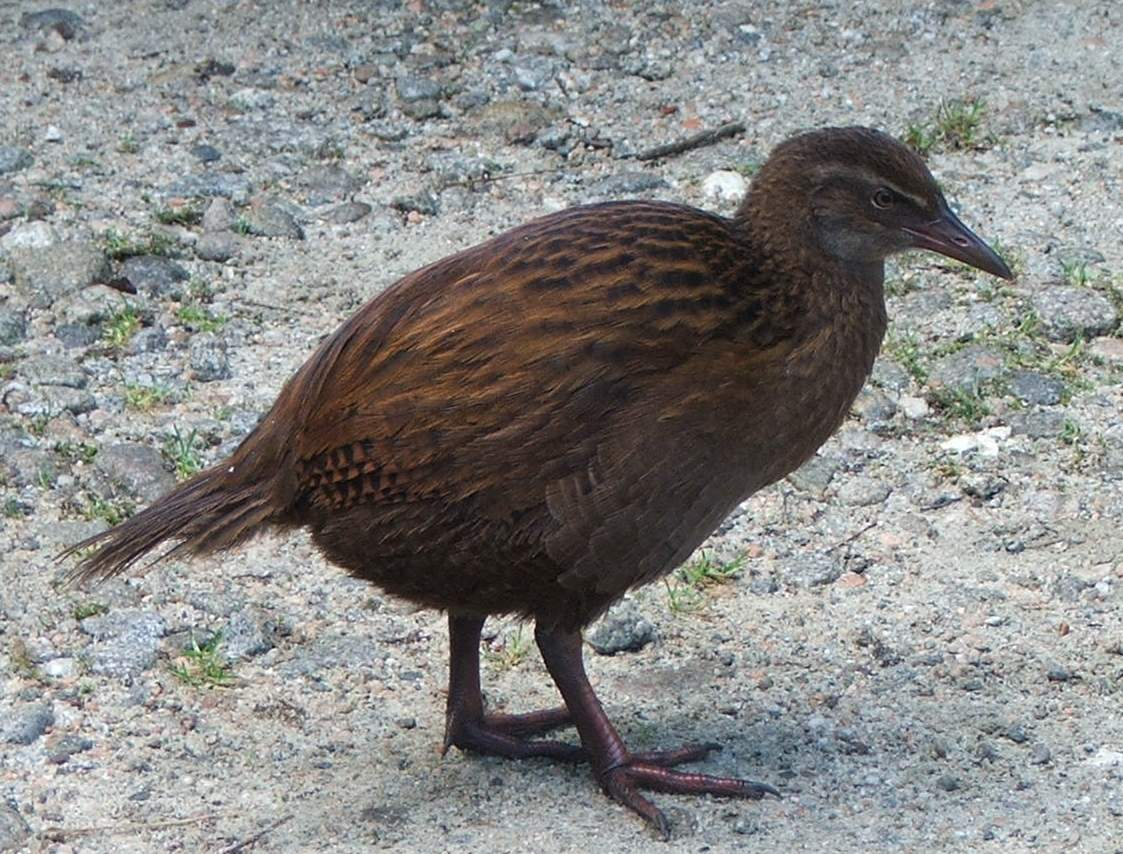
\includegraphics[scale=0.2]{SI_Weka.jpg}
\end{figure}

Можно послушать, как она поёт, \url{http://www.cs.waikato.ac.nz/ml/weka/sounds/weka-long.au}.


Однако при загрузке пакета нужно убедиться, что на компьютере установлена среда Java, и~отдавать себе отчёт, что поиск подходящих параметров и~пятикратная оценка классификатора будет требовать значительного времени.

Используем функцию \code|IBk|. 
Для этого добавим слева к~нашей матрице \code|train| столбец с~ответами и~преобразуем матрицу в~объект \code|data.frame|. 
Выражение \code|K = 10| указывает на то, что алгоритм будет перебирать все значения от~1 до~10. 
Функция \code|evaluate_weka_classifier| оценивает качество результатов и~показывает, какие значения были классифицированы правильно в~результате пятикратного разбиения выборки на кусочки и~последующего усреднения, а~какие "--- нет. 

Обратите внимание на \ENGs{Confusion matrix}, которая показывает, с~какими именно классами возникали ошибки: можно заметить, что пятёрки и~восьмёрки классифицировались как всё что угодно.

\begin{knitrout}
\definecolor{shadecolor}{rgb}{0.969, 0.969, 0.969}\color{fgcolor}\begin{kframe}
\begin{alltt}
\hlkwd{library}\hlstd{(RWeka)}

\hlstd{train_weka} \hlkwb{<-} \hlkwd{data.frame}\hlstd{(train_labels, train)}
\hlstd{train_weka[,}\hlnum{1}\hlstd{]} \hlkwb{<-} \hlkwd{as.factor}\hlstd{(train_weka[,}\hlnum{1}\hlstd{])}
\hlstd{classifier} \hlkwb{<-} \hlkwd{IBk}\hlstd{(train_labels}\hlopt{~}\hlstd{.,} \hlkwc{data} \hlstd{= train_weka,}
                  \hlkwc{control} \hlstd{=} \hlkwd{Weka_control}\hlstd{(}\hlkwc{K} \hlstd{=} \hlnum{10}\hlstd{,} \hlkwc{X}\hlstd{=}\hlnum{TRUE}\hlstd{))}
\hlstd{classifier}
\end{alltt}
\begin{verbatim}
## IB1 instance-based classifier
## using 1 nearest neighbour(s) for classification
\end{verbatim}
\begin{alltt}
\hlkwd{evaluate_Weka_classifier}\hlstd{(classifier,} \hlkwc{numFolds} \hlstd{=} \hlnum{5}\hlstd{)}
\end{alltt}
\begin{verbatim}
## === 5 Fold Cross Validation ===
## 
## === Summary ===
## 
## Correctly Classified Instances         872               87.2    %
## Incorrectly Classified Instances       128               12.8    %
## Kappa statistic                          0.8576
## Mean absolute error                      0.0275
## Root mean squared error                  0.1591
## Relative absolute error                 15.2961 %
## Root relative squared error             53.0432 %
## Coverage of cases (0.95 level)          87.2    %
## Mean rel. region size (0.95 level)      10      %
## Total Number of Instances             1000     
## 
## === Confusion Matrix ===
## 
##    a   b   c   d   e   f   g   h   i   j   <-- classified as
##   91   0   0   0   0   0   5   0   0   1 |   a = 0
##    0 115   0   0   0   0   0   1   0   0 |   b = 1
##    2   4  80   1   0   2   2   4   1   3 |   c = 2
##    0   1   3  80   0   4   1   2   1   1 |   d = 3
##    0   5   0   0  86   1   1   1   0  11 |   e = 4
##    0   2   1   2   0  79   3   1   2   2 |   f = 5
##    1   3   0   0   0   0  88   0   1   1 |   g = 6
##    0   5   1   0   2   3   0 100   1   5 |   h = 7
##    0   3   2   2   2   5   2   0  69   2 |   i = 8
##    1   1   0   0  10   1   1   1   1  84 |   j = 9
\end{verbatim}
\end{kframe}
\end{knitrout}

Теперь предскажем значения для тестовой выборки с~помощью функции \code|predict| и~посмотрим на долю ошибок.

\begin{knitrout}
\definecolor{shadecolor}{rgb}{0.969, 0.969, 0.969}\color{fgcolor}\begin{kframe}
\begin{alltt}
\hlstd{test_weka} \hlkwb{=} \hlkwd{data.frame}\hlstd{(test)}
\hlkwd{names}\hlstd{(test_weka)} \hlkwb{=} \hlkwd{names}\hlstd{(train_weka)[}\hlopt{-}\hlnum{1}\hlstd{]}

\hlstd{predictions} \hlkwb{<-} \hlkwd{predict}\hlstd{(classifier,} \hlkwc{newdata} \hlstd{= test_weka)}

\hlstd{errors} \hlkwb{<-} \hlstd{(}\hlkwd{sum}\hlstd{(predictions} \hlopt{!=} \hlstd{test_labels))}\hlopt{/}\hlstd{m}
\hlstd{errors}
\end{alltt}
\begin{verbatim}
## [1] 0.174
\end{verbatim}
\end{kframe}
\end{knitrout}

\section{Заключение}

Таким образом, мы рассмотрели интересную задачу и~отличную, заботливо собранную базу данных, применили к~ним один из самых первых и~простых алгоритмов машинного обучения, который, однако, часто показывает очень хорошие результаты. 
Но это был один только пример, а~в~качестве инструментов в~данном случае могут быть использованы разнообразнейшие алгоритмы. 
Кроме того, можно подумать над тем, как преобразовать сами изображения для улучшения качества классификации. Удачи!


\printbibliography


\end{document}
